\subsubsection{\gls{KA}}

\textbf{Ansvar} \\
Kasseapparatet er den del af systemet hvor produktkataloget bliver vist og benyttet til salg af produkter. Her i bliver vist en liste/indkøbskurv med de produkter som en evt. kunde ønsker at købe, samt dannet salgskvitteringer for gennemførte salg. Produktkataloget bliver hentet ved en forespørgsel til Centralserver og kasseapparatet ved derved intet om oprettelse og redigering af de produkter som den fremviser. \\

\textbf{Sekvensdiagram}
\begin{figure}[H]
	\centering
	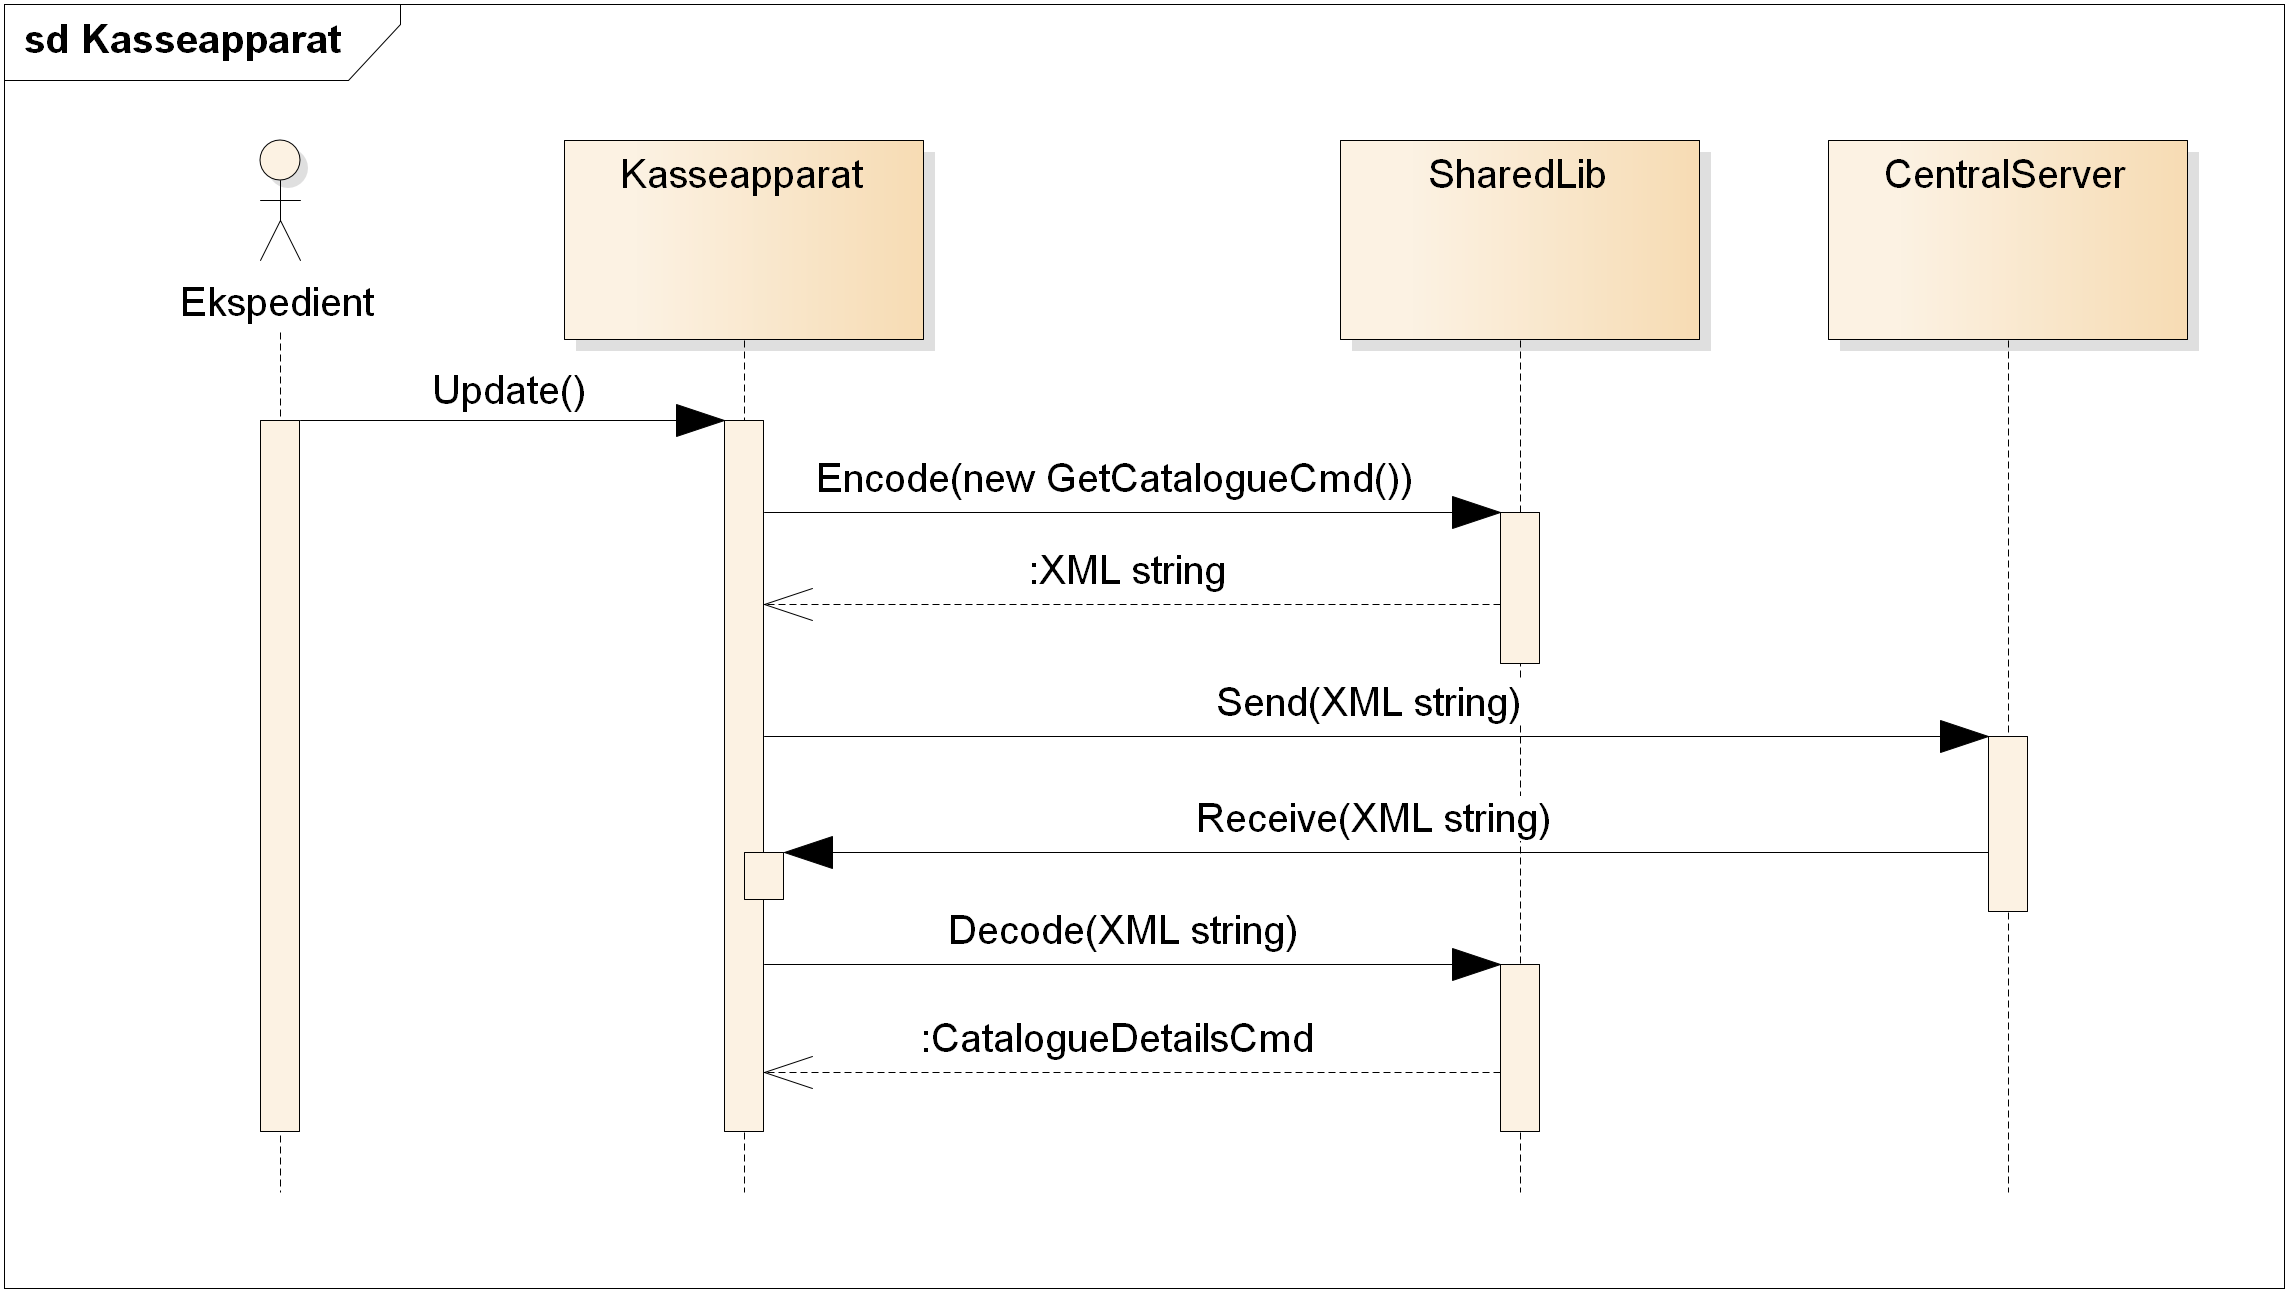
\includegraphics[scale=0.7]{Systemarkitektur/LogiskView/Kasseapparat-sekvensdiagram}
	\caption{Sekvensdiagram for kommunikation mellem \gls{KA} og andre pakker}
	\label{fig:logview_kasse_sekvensdiagram}
\end{figure}

Sekvensdiagrammet viser hvordan kasseapparatet kommunikerer med de andre pakker i systemet. Kasseapparatet kommunikerer udelukkende med den centrale server. Når kasseapparatet skal sende en besked til CentralServer bruger den SharedLib til at konvertere et kommando objekt til en XML string og sender herefter denne til CentralServeren. Der modtages herefter en XML string, som respons, som så derefter bliver decoded til et kommando objekt, igen ved brug af SharedLib.

\newpage
